\subsection{Experiments: DFR at 20-bit security}


\begin{frame}{Our approach (joint with Arpin, Bilingsley, Hast, Perlner, Robinson) }
    \begin{itemize}
        \item Compute average DFR using simulations for security level $\lambda= 20$.
        \item Study contributing factors: classes of weak keys, sets of problematic error patterns, properties of decoders.
    \end{itemize}
\end{frame}



\begin{frame}{20-bit DFR experiments}
        \begin{itemize}
        \item BIKE security specifications require DFR $< 2^{-\lambda}$ for security levels $\lambda = 128,192,256$.
        \item $\lambda = 20$-bit parameters:
        \begin{itemize}
            \item column weight $w/2 = 30$;
            \item error weight $t = 18$;
            \item block size $r \in [389,827]$.
        \end{itemize}
        \item To achieve $\lambda$ bits of security against information set decoding:
        
        \[\lambda \approx t - \frac{1}{2}log_2 r \approx w - log_2 r.
        \]
    \end{itemize}
\end{frame}

\begin{frame}{20-bit DFR experiments}
We ran the simulation on Boston University's Shared Computing Cluster.

\begin{columns}

\column{0.5 \textwidth}
\begin{enumerate}
    \item Generate a random parity check matrix $H$, an error vector $e$.
    \item Compute the syndrome $s = He^T$.
    \item Run the BGF decoder on inputs $H,s$.
    \item Record decoding failures.
\end{enumerate}

\column{0.5 \textwidth}
\begin{figure}
    \centering
    \includegraphics[scale=.12]{Images/buscc.jpg}
\end{figure}
\end{columns}

\end{frame}

\begin{frame}{20-bit DFR experiments}

\begin{columns}

\column{0.5 \textwidth}
\begin{itemize}
    \item Tested $10^8, 10^9$ for $r \in [389, 827]$.
    \item Plotted with 95\% confidence interval.
    \item Fit lines are quadratic for waterfall region and linear for error floor region.
\end{itemize}

\column{0.5 \textwidth}
\begin{figure}
    \centering
    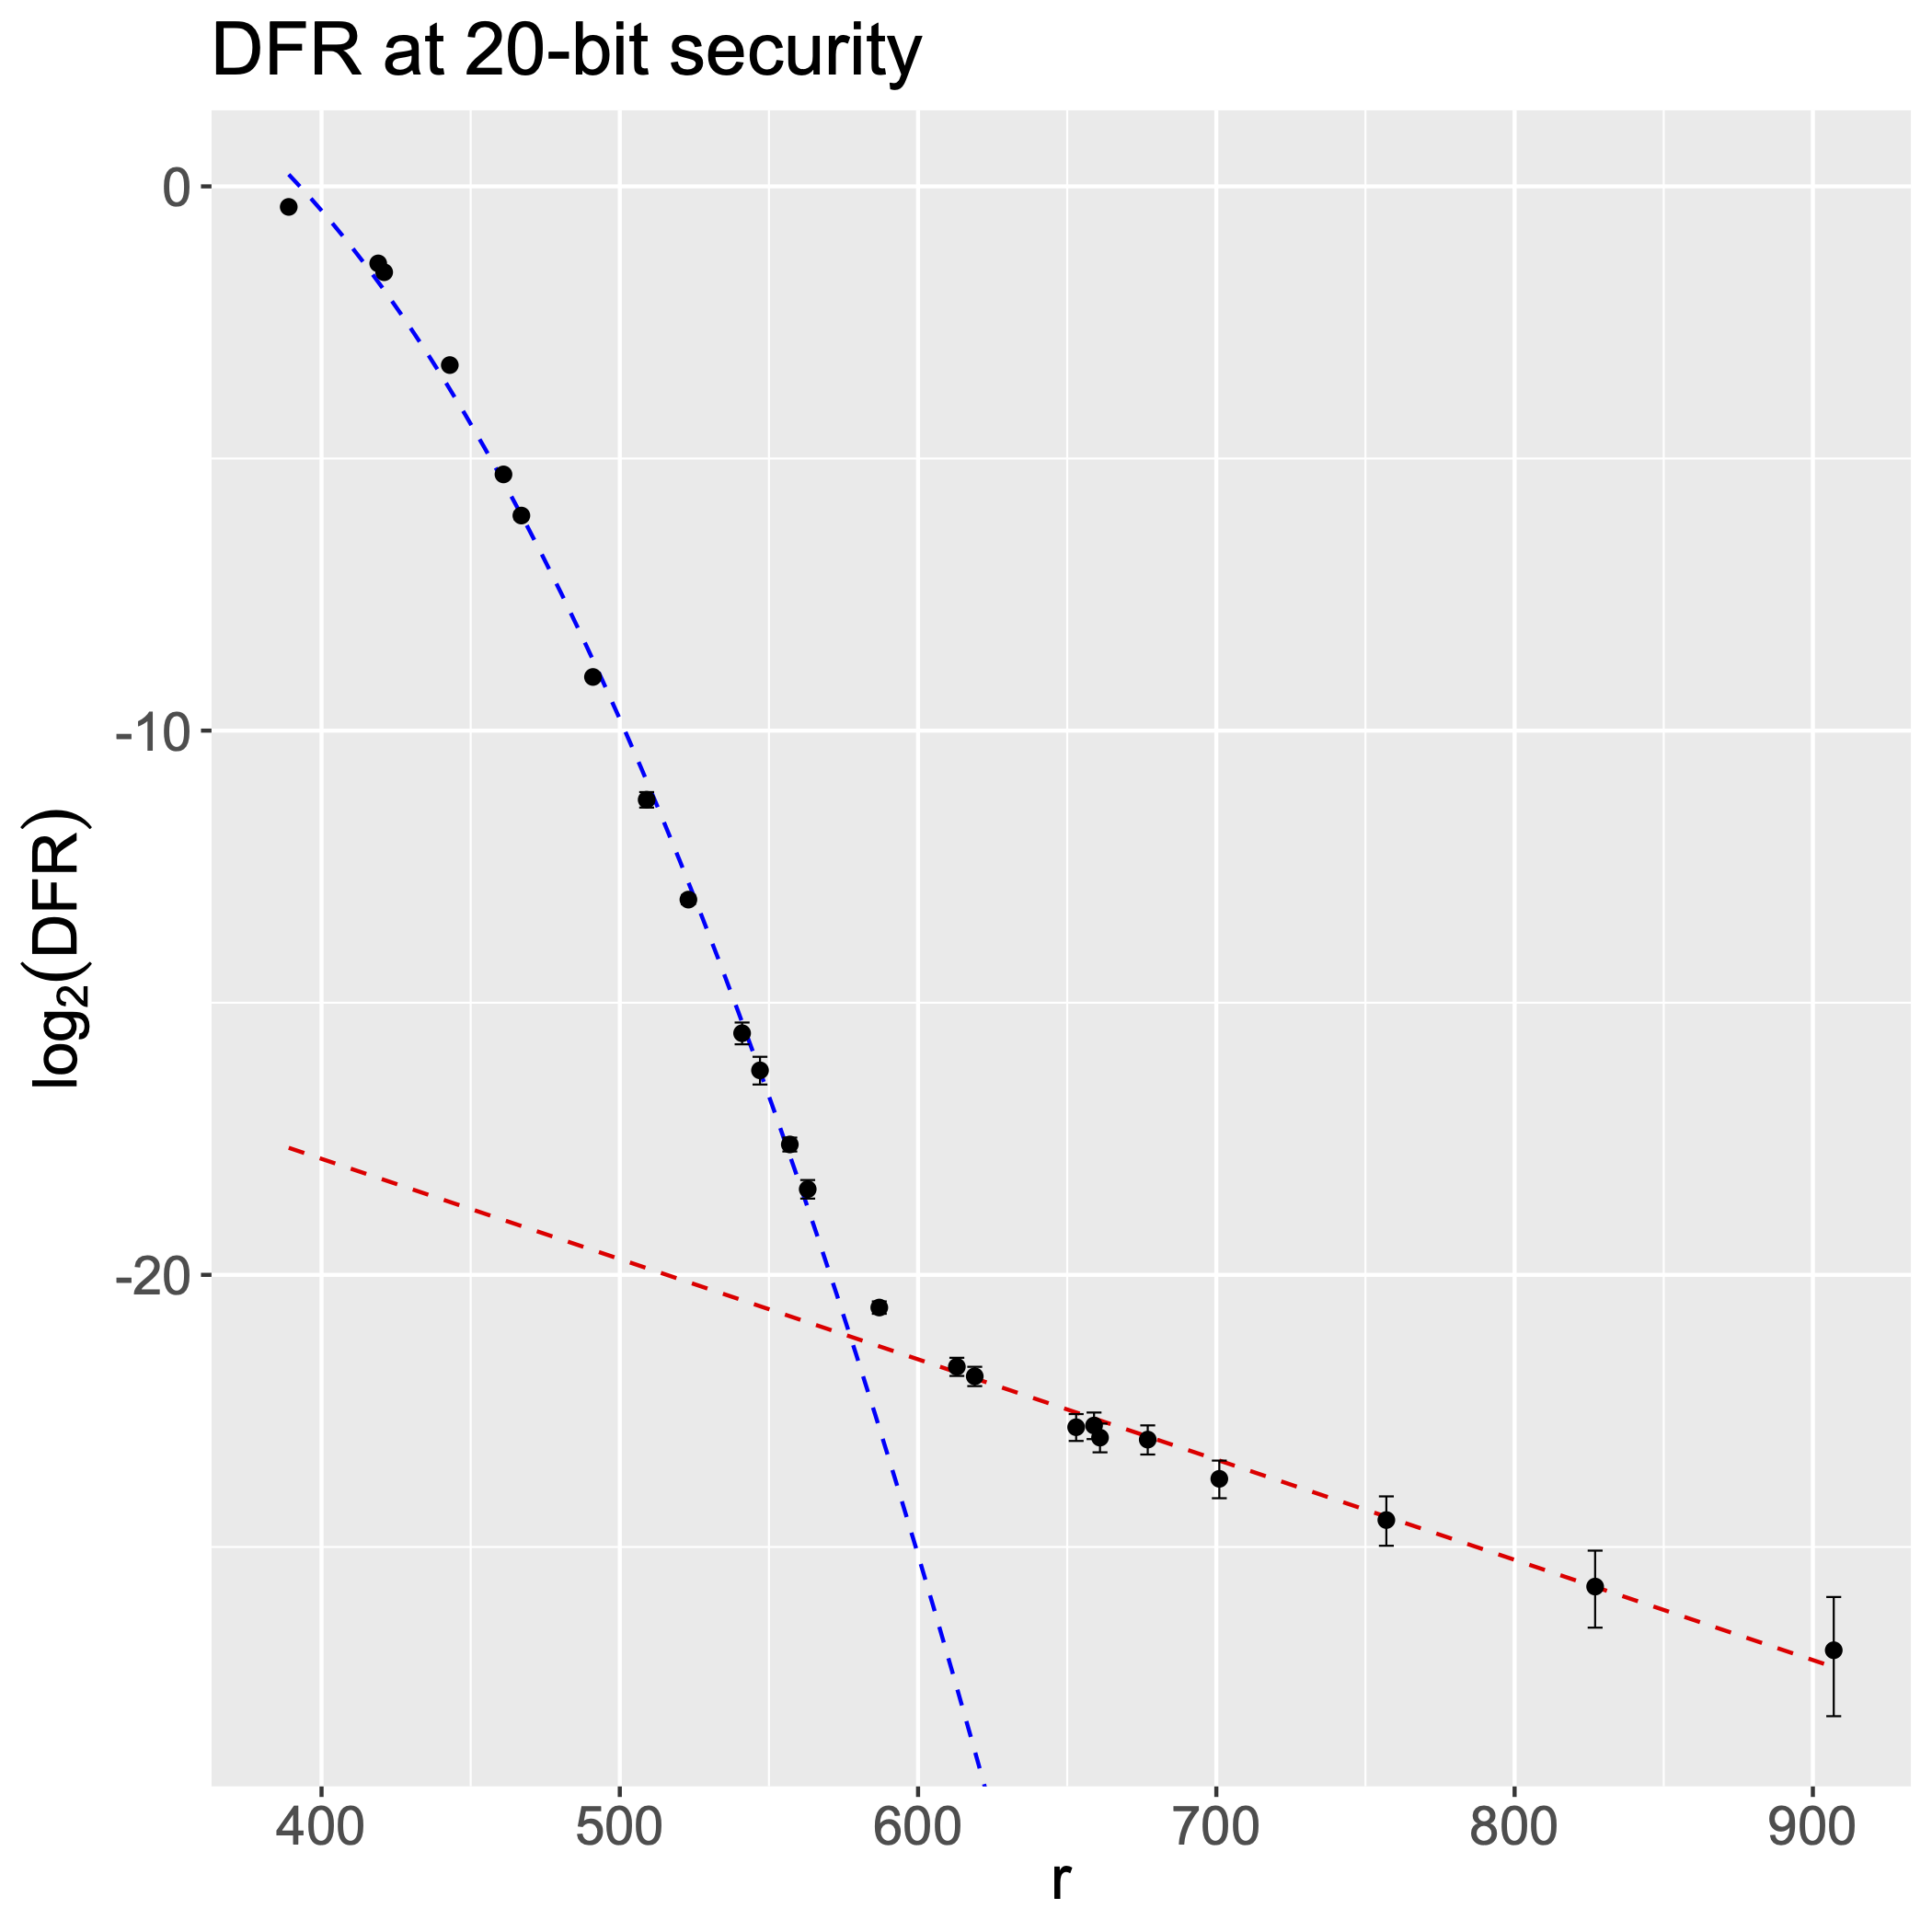
\includegraphics[scale=.07]{Images/DFR-plot-T3.png}
\end{figure}

\end{columns}
    
\end{frame}

\begin{frame}{Problematic error vectors}
In syndrome decoding, one issue can arise:

\begin{block}{Problem}
Given $H,s$, we may get $e_1$,$e_2$ such that:
     \[  He_1^T = s = He_2^T \iff e_1- e_2 \in C\]

    
\end{block}
Richardson considered \textbf{$(u,v)$ near-codewords}: error vectors $|e| = u$ such that $|He^T| = v$. 
    
    \begin{itemize}
        \item With $u,v$ small relative to $n$, the decoder might be trapped and return $|x| \leq t$ but $Hx^T = s$.
    \end{itemize}
    

\end{frame}


\begin{frame}{Problematic error vectors}

    Following Richardson, Vasseur identified $3$ problematic sets of error vectors:

    \begin{itemize}
        \item $\mathcal{C}$: the set of weight $w$ codewords;
        \item $\mathcal{N}$: the set of half rows of $H$;
        \item $2\mathcal{N}$: the set of sum of two elements of $\mathcal{N}$.
    \end{itemize}
    
    Idea:
    \begin{itemize}
        \item Correspond to Richardson's low weight codewords and $(u,v)$ near-codewords.
        \item Vectors close to $\mathcal{S}$ are more likely to be indistinguishable in the syndrome decoding problem.
    \end{itemize}

    
\end{frame}

\begin{frame}{Problematic error vectors}
        For $\mathcal{S} \in \{ \mathcal{C},\mathcal{N}, 2\mathcal{N}\}$, Vasseur defines:
    
    \[
    \mathcal{A}_{t,\ell}(\mathcal{S}) = \bigcup_{v \in \mathcal{S}} \{ e \in \FF_2^n| |e| = t, |e \star v| = \ell \}.
    \]
    
    If $e \in \mathcal{A}_{t,\ell}(\mathcal{S})$, there exists $v\in \mathcal{S}$ such that $|e \star v| = \ell$. We define the distance $\delta:= |v| + t - 2\ell$.
    
\end{frame}



\begin{frame}{DFR for special sets}
    For $r = 523,587,659$, we computed DFR on $\mathcal{A}_{18,\ell}(\mathcal{S})$ for various $\delta$.
    
    \begin{block}{Question}
    How does the DFR of $t \in \mathcal{A}_{18,\ell}(\mathcal{S})$ compare to the DFR of generic vectors $|e| = 18$ ?
    \end{block}
\end{frame}

\begin{frame}{DFR for special sets}
    \begin{figure}
    \centering
    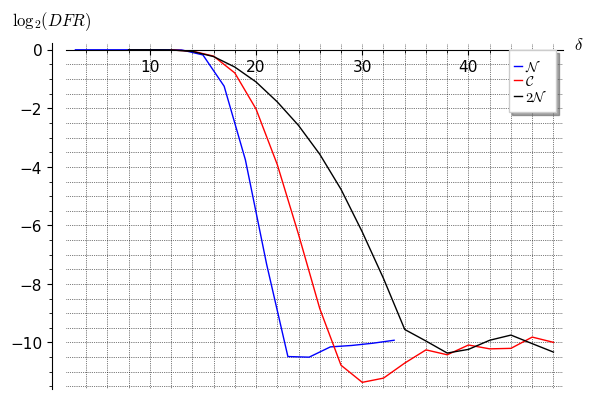
\includegraphics[scale=.6]{Images/DFR_20bit_CN2N_new.png}
    \caption{DFR vs $\delta$ for $r=587$}
\end{figure}

\end{frame}

\begin{frame}{Problematic vs generic error vectors}
    
    In our experiments, we recorded decoding failures. 
    
    \begin{block}{Question}
    How many overlaps do decoding failure vectors have with $\mathcal{C},\mathcal{N}, 2\mathcal{N}$?
    \end{block}
    
    For $r = 587$, we found the maximum number of overlaps with $\mathcal{S} \in \{\mathcal{C},\mathcal{N}, 2\mathcal{N} \} $ for each decoding failure vector. We repeat the experiment with random vectors and compare. 
    
\end{frame}


\begin{frame}{Problematic vs generic error vectors - data.}
\begin{columns}
    \column{0.5 \textwidth}
    \begin{figure}
    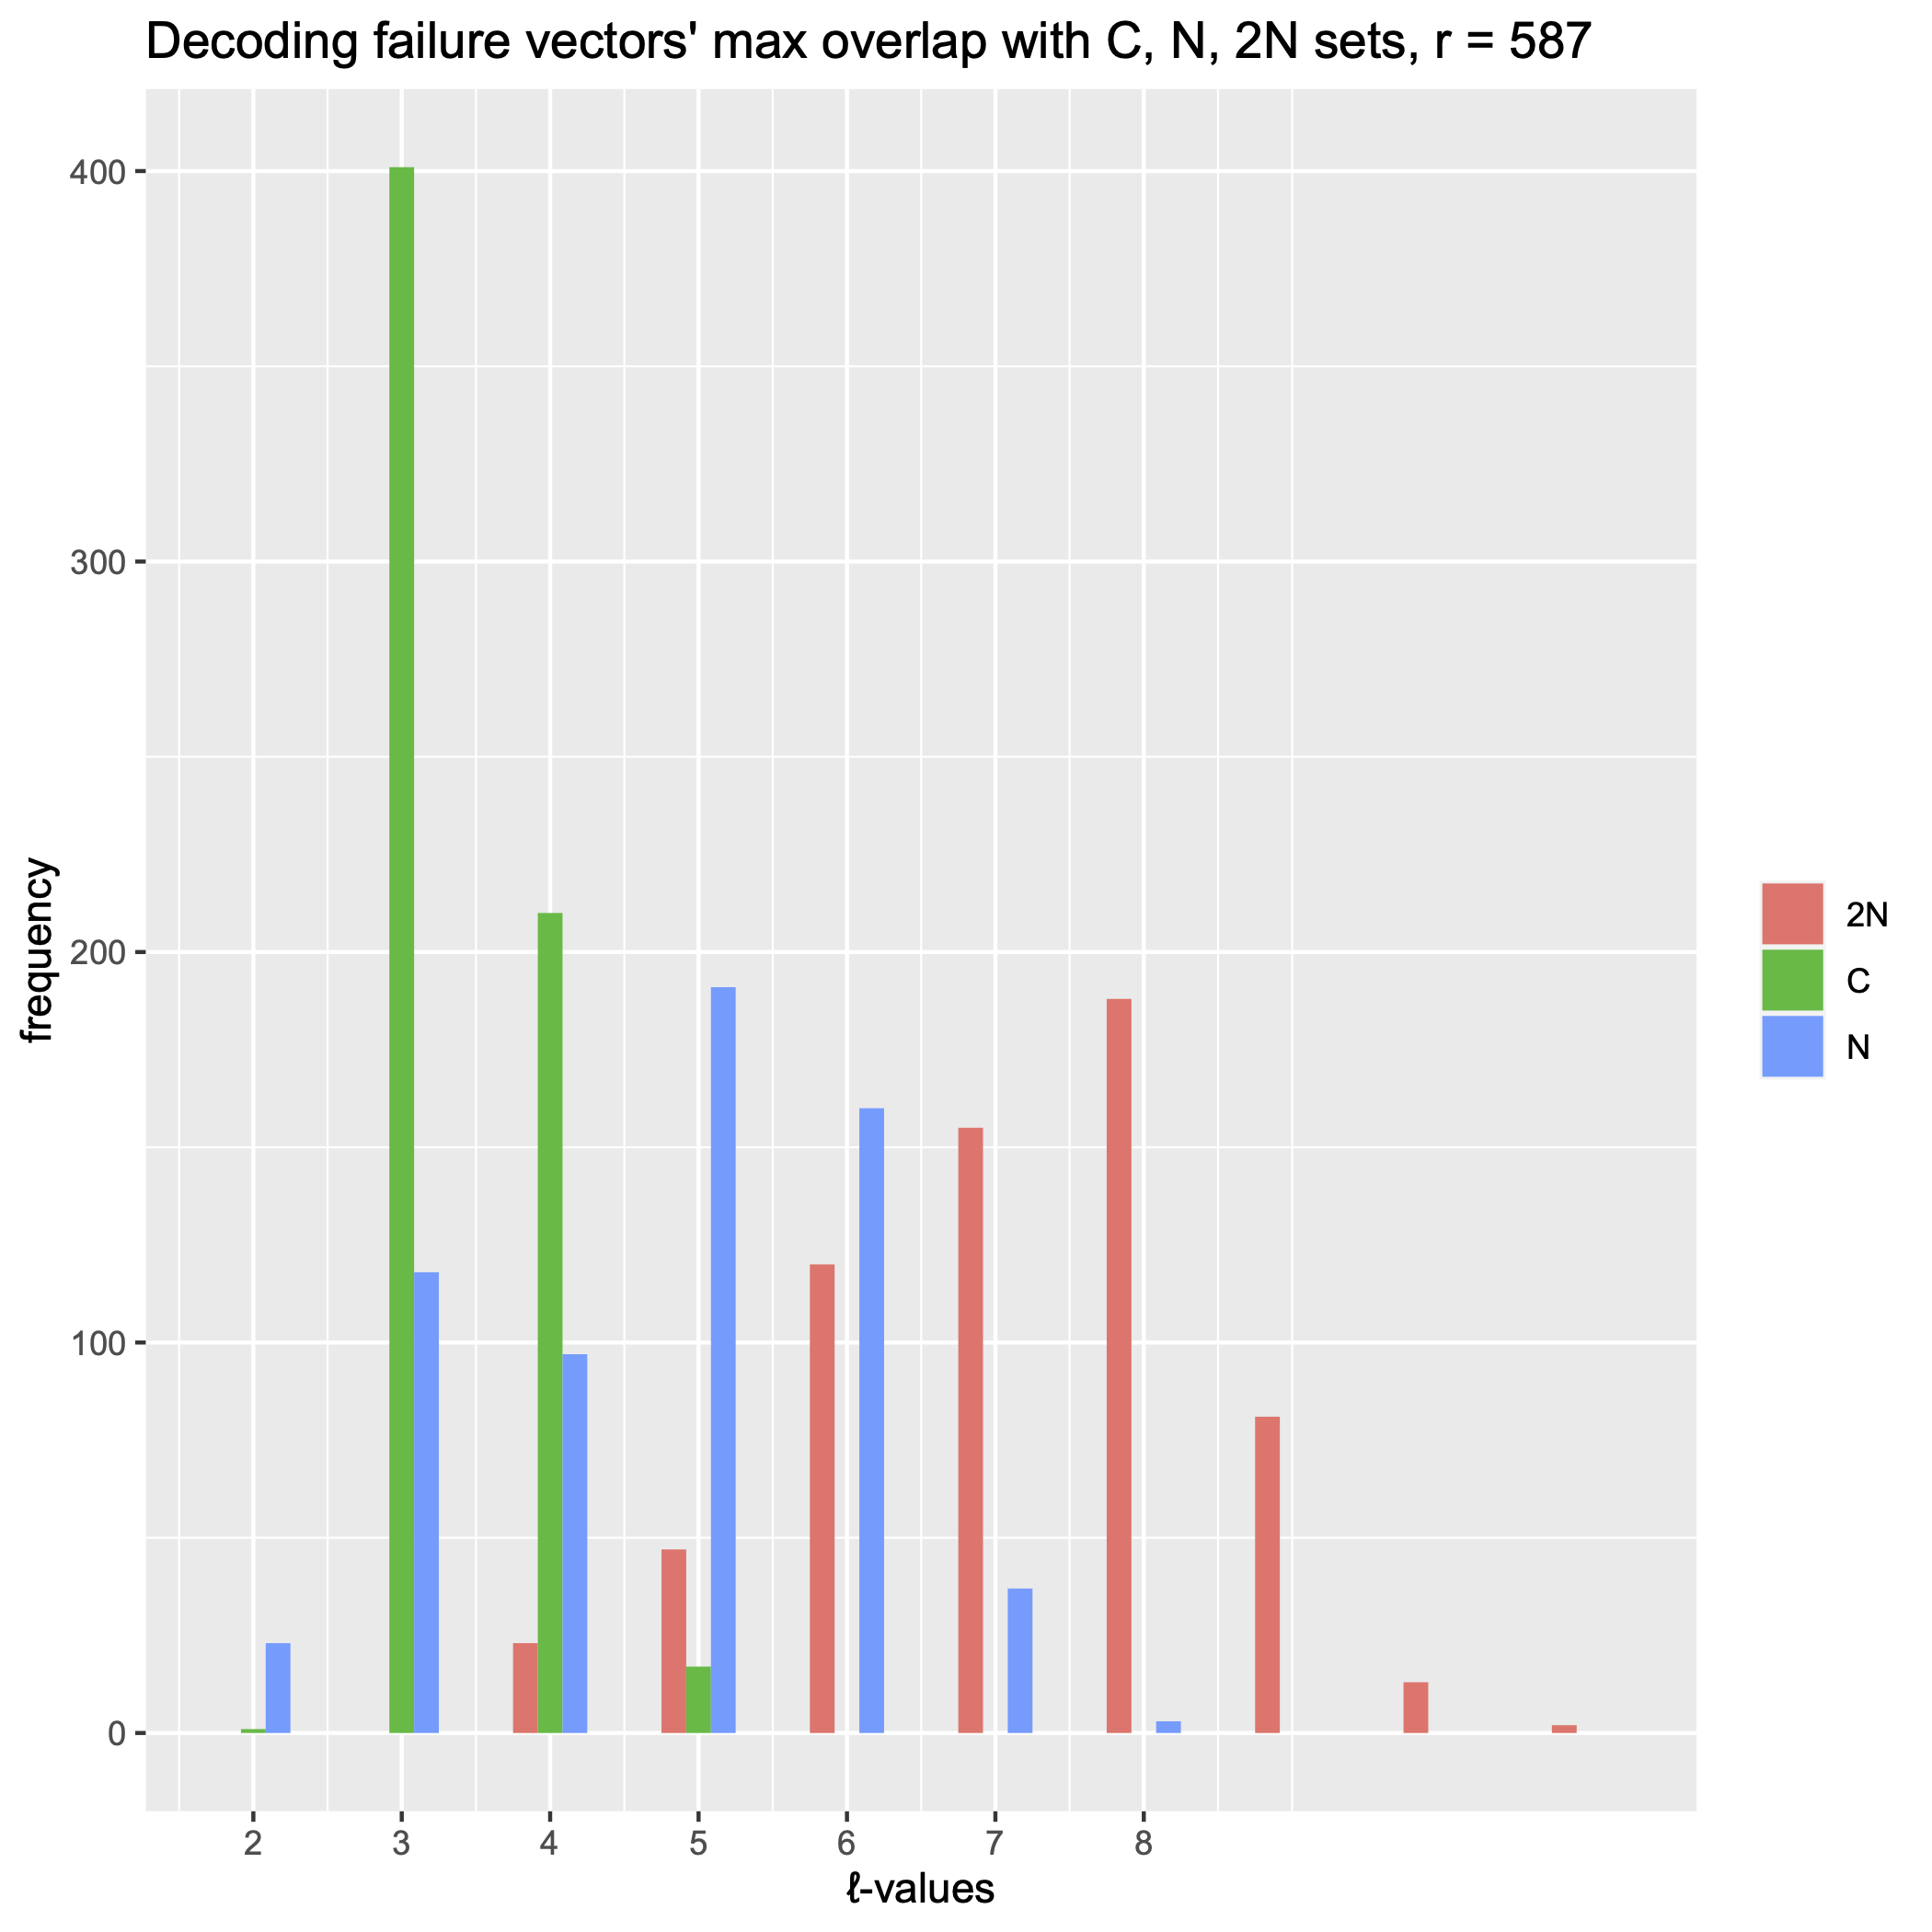
\includegraphics[scale=.06]{Images/Rplot-587-df.png}
    \caption{Decoding failure vectors}
    \end{figure}
    
    \column{0.5 \textwidth}
    \begin{figure}
    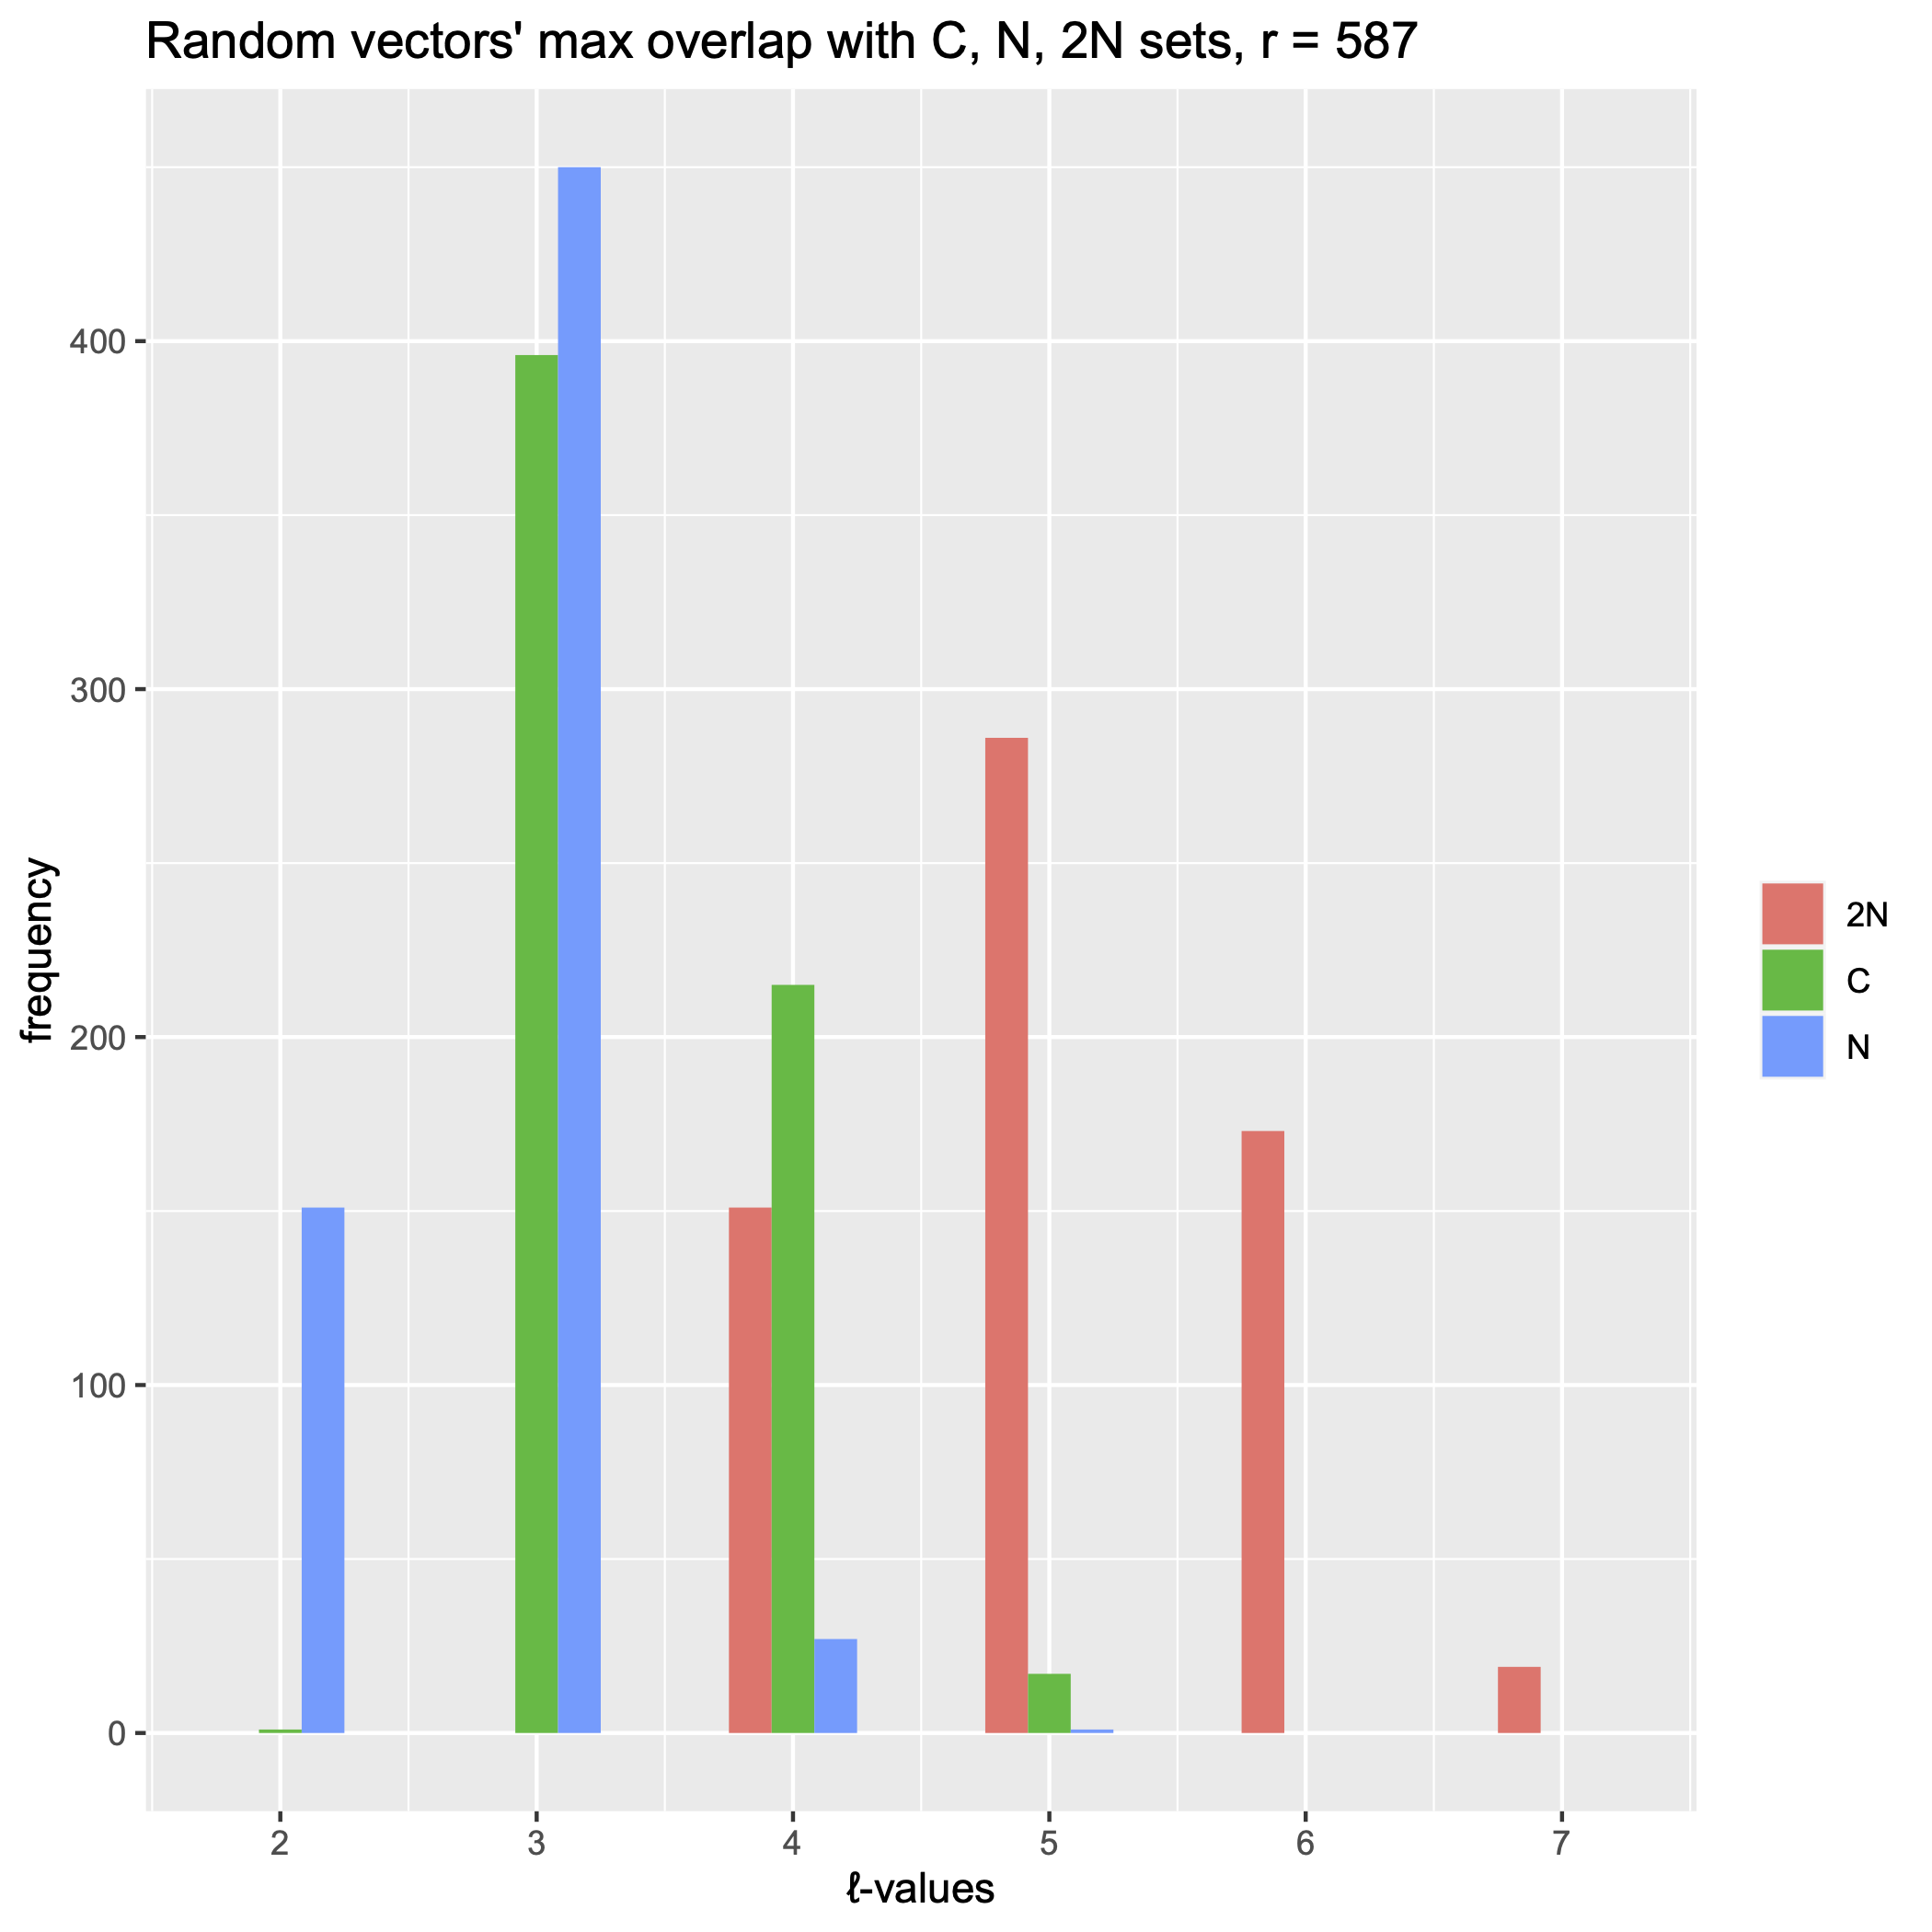
\includegraphics[scale=.06]{Images/Rplot-587-random.png}
    \caption{Randomly generated vectors}
    \end{figure}
\end{columns}

\begin{itemize}
\item Some proportion of decoding failures can be attributed to $\mathcal{N}, 2\mathcal{N}$.
\item A significant proportion of decoding failures do not have more overlap than typical random vectors.
\end{itemize}
\end{frame}

\begin{frame}{Syndrome weights of decoding failure vectors}
    From the DFR experiments of $\mathcal{A}_{t,\ell}(\mathcal{S})$, we observed that syndrome weights is an indicator of decoding failure.
    
    \begin{figure}
        \centering
        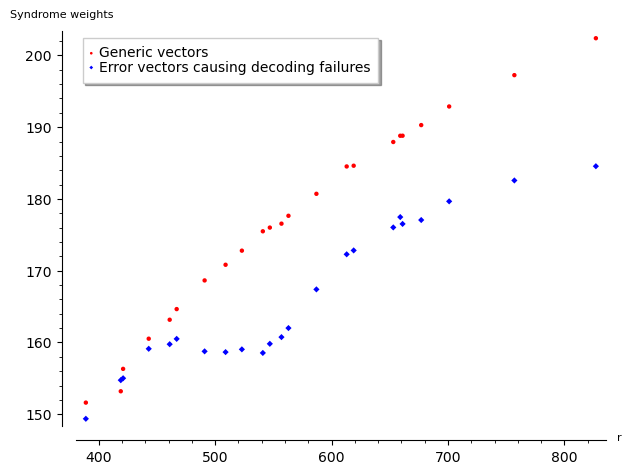
\includegraphics[scale=0.6]{Images/average_sw_generic_vs_DF_T3.png}
    \end{figure}
\end{frame}

\begin{frame}{Ongoing work}
    \begin{itemize}
        \item Apply graph theoretic techniques to study Tanner graphs of QC-MDPC codes.
\item Decoder behaviour (e.g., trapping sets, absorbing sets, etc.)
\item Syndrome weight and error floor phenomenon
    \end{itemize}
\end{frame}